\documentclass[10pt]{article}
\usepackage{graphicx}
\usepackage{amssymb}
\usepackage[fleqn]{amsmath}
\usepackage{nccmath}
\usepackage{cases}
\usepackage{hyperref}
\usepackage{multicol}
\usepackage{pgfplots}
\usepackage{enumitem}
\pgfplotsset{compat=1.18}
\usepackage{float}
\usepackage{pdfpages}
\DeclareMathOperator*{\argmax}{argmax\,}
\DeclareMathOperator*{\argmin}{argmin\,}

\title{\bf Math 156: Problem Set 1}
\author{\bf Owen Jones}
\begin{document}
\maketitle
\begin{enumerate}
    \item Given $D=\{x_1,x_2,\ldots,x_n\}$ is i.i.d, $\displaystyle p(D|\mathbf{w})=\prod_{i=1}^{n}p(x_i|\mathbf{w})$.
    \begin{align*}
        &\lambda_{ML}=\underset{\lambda}{\argmax}p(D|\lambda)
        =\underset{\lambda}{\argmax}\prod_{i=1}^{n}p(x_i|\lambda)
        =\underset{\lambda}{\argmax}\prod_{i=1}^{n}\frac{\lambda^{x_i}}{x_i!}e^{-\lambda}\\
        &=\underset{\lambda}{\argmax}\log(\prod_{i=1}^{n}\frac{\lambda^{x_i}}{x_i!}e^{-\lambda})
        =\underset{\lambda}{\argmax}\sum_{i=1}^{n}\log(\frac{\lambda^{x_i}}{x_i!}e^{-\lambda})\\
        &=\underset{\lambda}{\argmax}\sum_{i=1}^{n}x_i\log(\lambda)-\log(x_i!)-\lambda\\
        &=\underset{\lambda}{\argmax}-n\lambda+\log(\lambda)\sum_{i=1}^{n}x_i-\sum_{i=1}^{n}\log(x_i!)\\
        &\Leftrightarrow \frac{d \log(p(D|\lambda))}{d\lambda}=-n+\frac{1}{\lambda}\sum_{i=1}^{n}x_i=0\\
        &\Rightarrow n=\frac{1}{\lambda}\sum_{i=1}^{n}x_i\Rightarrow \lambda_{ML}=\frac{1}{n}\sum_{i=1}^{n}x_i
    \end{align*}
    \item \begin{align*}
        &\mathbf{w}_{ML}=\underset{\mathbf{w}}{\argmax}p(\mathbf{t}|\mathbf{x},\mathbf{x},\beta)
        =\underset{\mathbf{w}}{\argmax}\prod_{n=1}^{N}\mathcal{N}(t_n|y(x_n,\mathbf{w}),\beta^{-1})\\
        &=\underset{\mathbf{w}}{\argmax}\prod_{n=1}^{N}\frac{\sqrt{\beta}}{\sqrt{2\pi}}e^{-\frac{\beta}{2}{(t_n-y(x_n,\mathbf{w}))}^2}\\
        &=\underset{\mathbf{w}}{\argmax}\log(\prod_{n=1}^{N}\frac{\sqrt{\beta}}{\sqrt{2\pi}}e^{-\frac{\beta}{2}{(t_n-y(x_n,\mathbf{w}))}^2})\\
        &=\underset{\mathbf{w}}{\argmax}\frac{n}{2}\log(\frac{\beta}{2\pi})-\frac{\beta}{2}\sum_{n=1}^{N}{(t_n-y(x_n,\mathbf{w}))}^2\\
        &\text{the constant }\frac{n}{2}\log(\frac{\beta}{2\pi})\text{ doesn't change minimizer }\mathbf{w}_{ML}\\
        &\argmax f(x)=\argmin-f(x) \text{ thus:}\\
        &\Leftrightarrow \underset{\mathbf{w}}{\argmin} E(\mathbf{w})=\underset{\mathbf{w}}{\argmin}\frac{\beta}{2}\sum_{n=1}^{N}{(t_n-y(x_n,\mathbf{w}))}^2\\
        &\Leftrightarrow \nabla E(\mathbf{w})=0\Rightarrow \frac{\partial E(\mathbf{w})}{\partial i}=0\text{ by FONC}\\
        &\text{By Chain Rule}\\
        &\frac{\partial E(\mathbf{w})}{\partial w_i}=\beta\sum_{n=1}^{N}{(t_n-y(x_n,\mathbf{w}))}x_n^i=\beta\sum_{n=1}^{N}{(t_n-\sum_{j=0}^{M}w_j x_n^j)}x_n^i=0\\
        &\Rightarrow \sum_{j=0}^{M}w_j\underbrace{\sum_{n=1}^{N} x_n^{i+j}}_{A_{ij}}=\underbrace{\sum_{n=1}^{N}t_n x_n^i}_{T_i}
    \end{align*}
    Hence, $\mathbf{w}_{ML}$ solves the set of linear equations $\displaystyle\sum_{j=0}^{M}A_{ij}w_j=T_i$
    \item Below is a pdf of my code including the function used to generate the curve of best fit and a graph with a scatterplot of the imported data and the curve of best fit for the chosen number of coefficients. 
    As $M$ increases, the upper bound for the relative error between the exact and numerical solution for $w$ grows exponentially. 
    Chose $M=8$ because there is a large decrease in the least square error between $M=7$ and $M=8$, and while the upper bound for the relative error is much larger than for $M=7$, it is significantly smaller than for any $M>8$.
    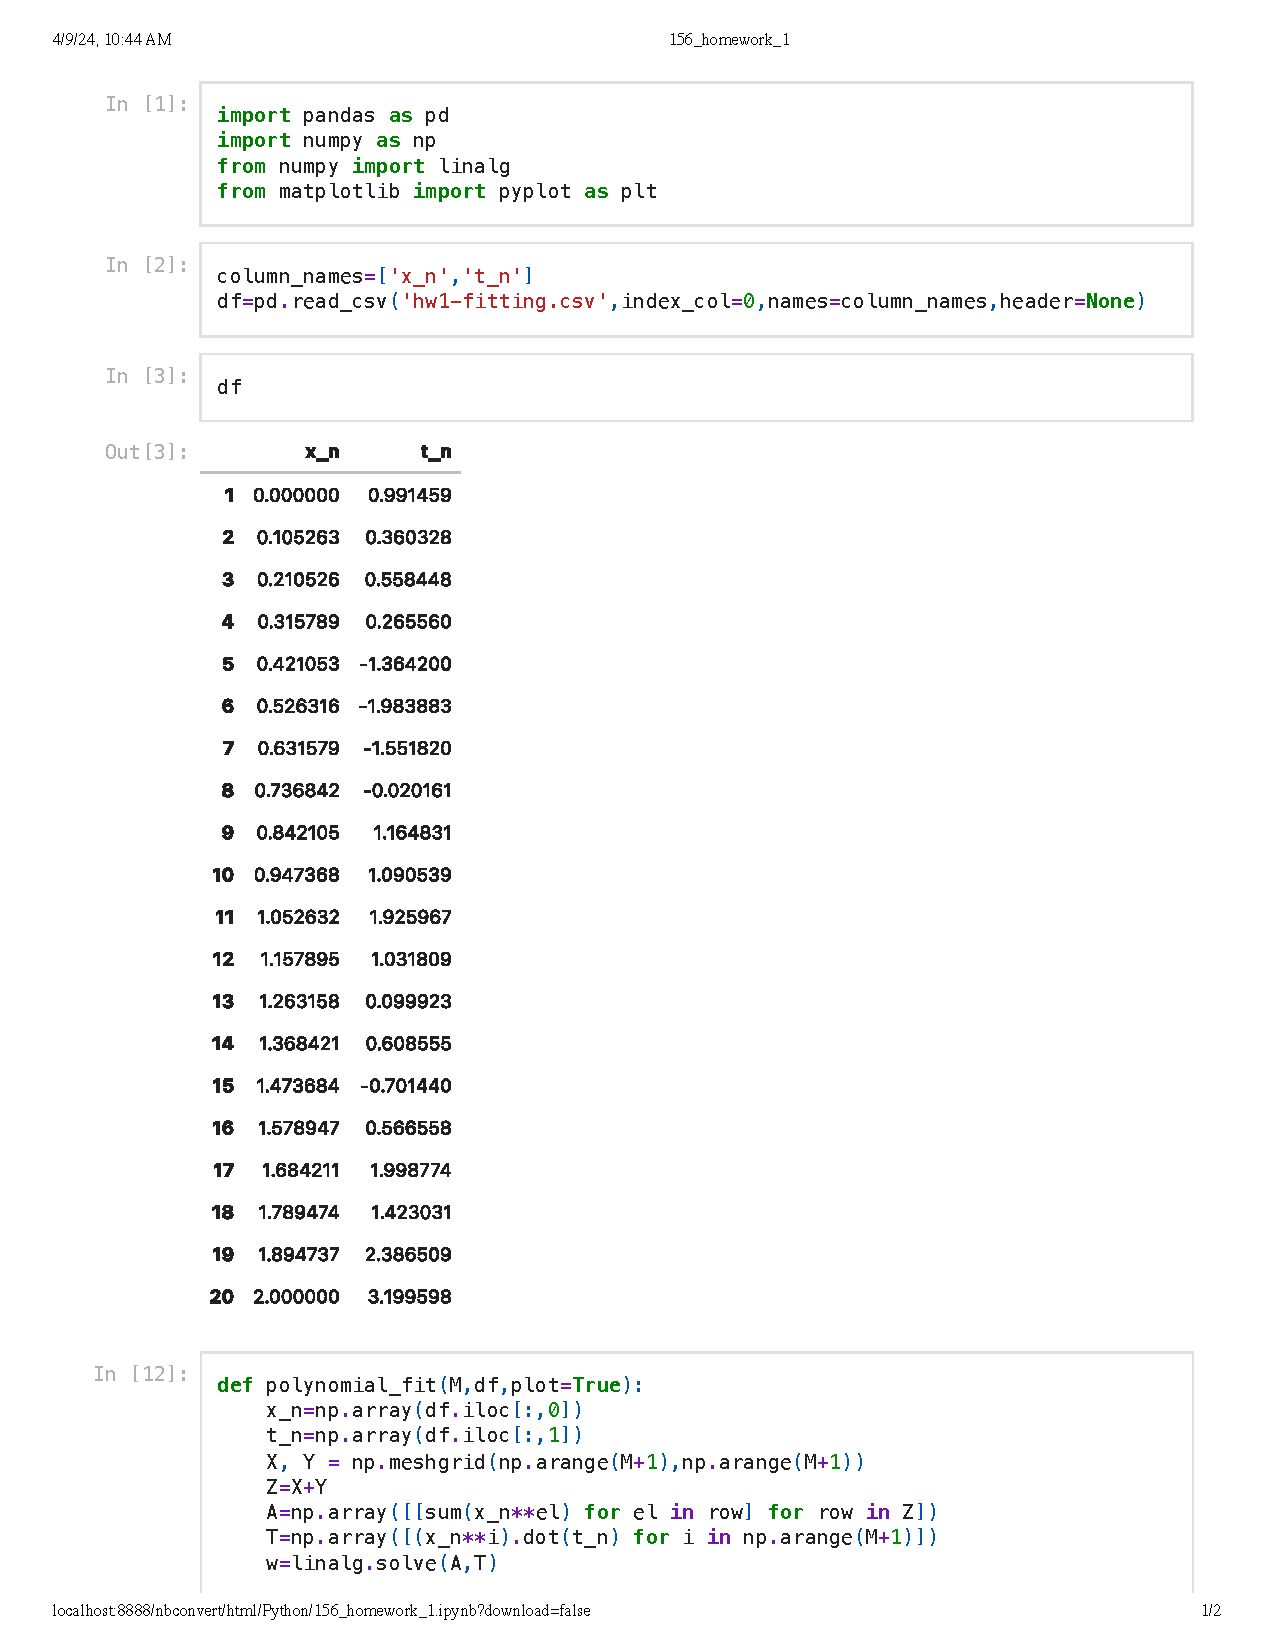
\includepdf[pages=-]{156_homework_1.pdf}
\end{enumerate}
\end{document}